\documentclass[tikz,border=0mm]{standalone}
\usepackage[utf8]{inputenc}
\usepackage{unicode-math} % for unicode support in math environments
\usepackage{amsmath}
\usepackage{siunitx}
\usepackage{booktabs}
\sisetup{mode=text,range-phrase = {\text{~to~}}, range-units=single, print-unity-mantissa=false}
\usepackage{mhchem}
\usepackage{tikz}



\usepackage{fontspec}

\directlua{
  luaotfload.add_fallback(
  "FallbackFonts",
  {
        "DejaVu Serif:mode=harf;",
        "DejaVu Sans Mono:mode=harf;",
        % we could add many more fonts here optionally!
    }
  )
}

\setmainfont{CMU Serif}[RawFeature={fallback=FallbackFonts}]
\setmonofont{Inconsolata}[RawFeature={fallback=FallbackFonts}]

\begin{document}
\definecolor{backgroundColor}{rgb}{1.0, 1.0, 1.0}

\pagecolor{backgroundColor}


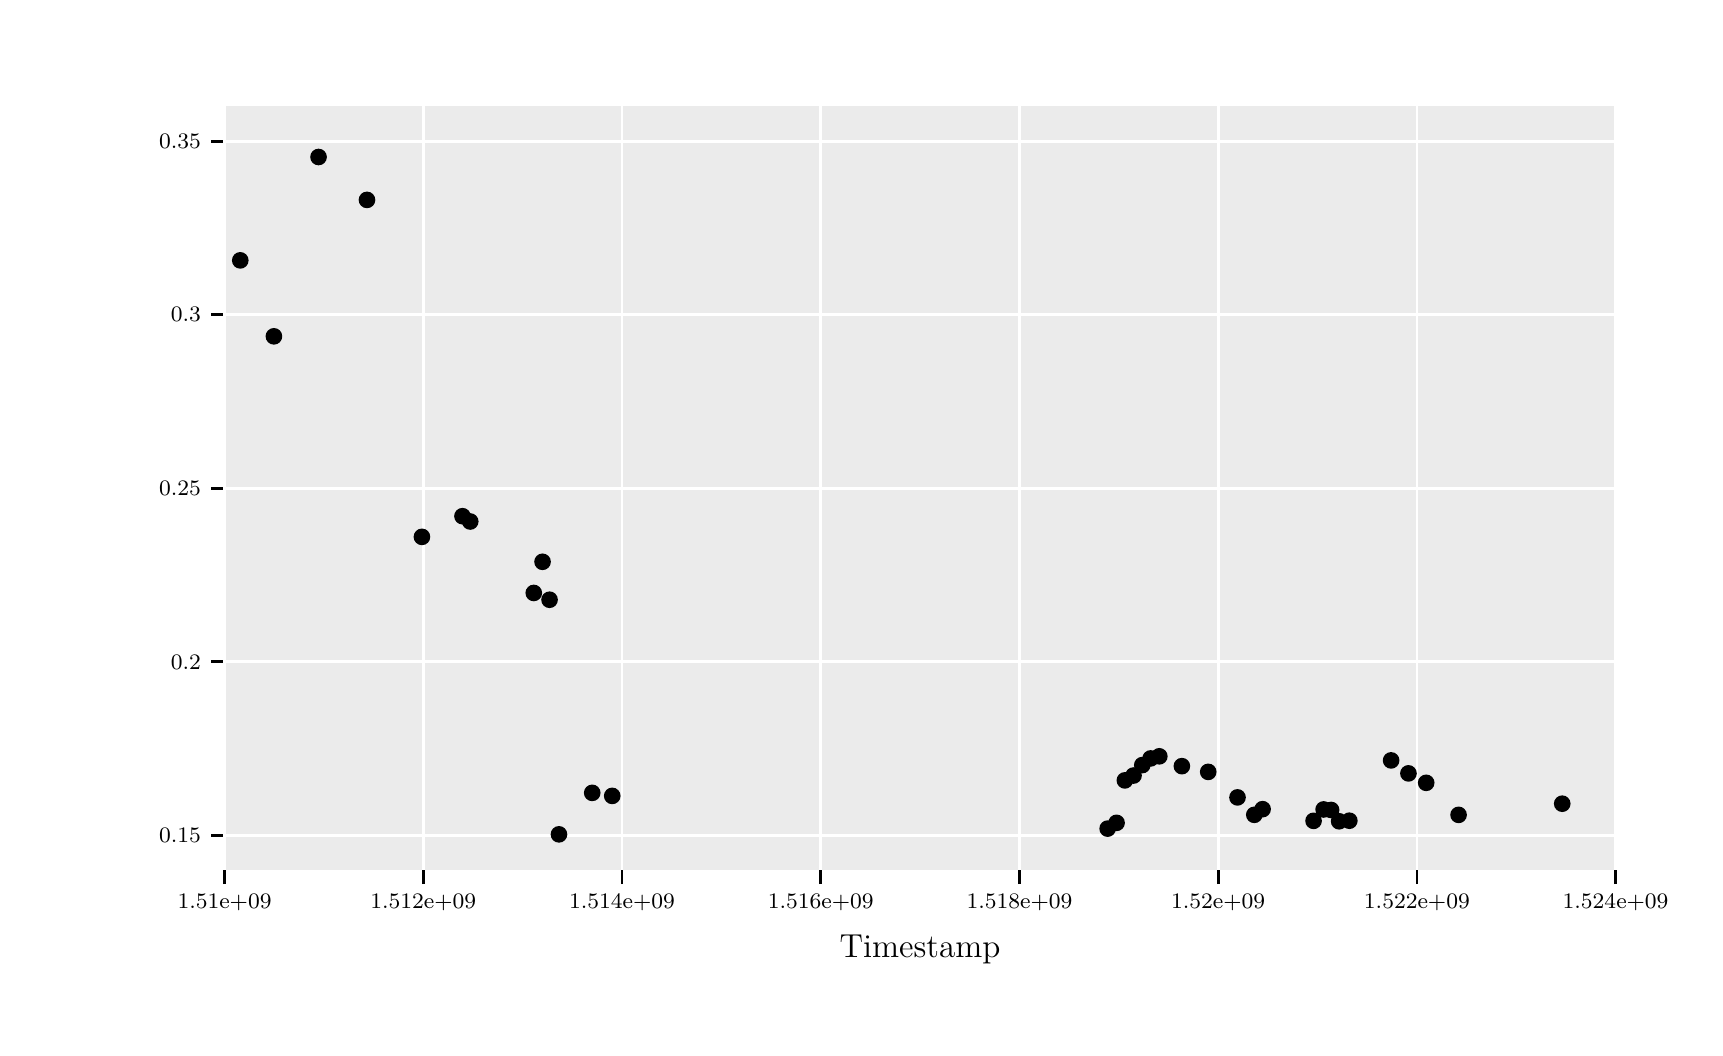
\begin{tikzpicture}[every node/.style={outer sep=0pt, inner sep=0pt}]
\path[use as bounding box] (0, 0) rectangle (600.0bp, 360.0bp) ;
\definecolor{drawColor}{rgb}{0.0, 0.0, 0.0}
\definecolor{fillColor}{rgb}{1.0, 1.0, 1.0}

\draw [color = drawColor, fill = fillColor, draw opacity = 0.0, fill opacity = 1.0, line width = 0.0bp] (0.0000bp, 360.0000bp) rectangle (600.0000bp, 0.0000bp) ;
\definecolor{drawColor}{rgb}{0.0, 0.0, 0.0}
\definecolor{fillColor}{rgb}{0.9200000166893005, 0.9200000166893005, 0.9200000166893005}

\draw [color = drawColor, fill = fillColor, draw opacity = 0.0, fill opacity = 1.0, line width = 0.0bp] (70.8661bp, 331.6535bp) rectangle (571.6535bp, 56.6929bp) ;
\definecolor{drawColor}{rgb}{0.0, 0.0, 0.0}
\definecolor{fillColor}{rgb}{0.0, 0.0, 0.0}

\draw [color = drawColor, fill = fillColor, draw opacity = 1.0, fill opacity = 0.0, line width = 1.0bp] (70.8661bp, 51.6929bp)--(70.8661bp, 56.6929bp) ;
\draw [color = drawColor, fill = fillColor, draw opacity = 1.0, fill opacity = 0.0, line width = 1.0bp] (142.4072bp, 51.6929bp)--(142.4072bp, 56.6929bp) ;
\draw [color = drawColor, fill = fillColor, draw opacity = 1.0, fill opacity = 0.0, line width = 1.0bp] (213.9483bp, 51.6929bp)--(213.9483bp, 56.6929bp) ;
\draw [color = drawColor, fill = fillColor, draw opacity = 1.0, fill opacity = 0.0, line width = 1.0bp] (285.4893bp, 51.6929bp)--(285.4893bp, 56.6929bp) ;
\draw [color = drawColor, fill = fillColor, draw opacity = 1.0, fill opacity = 0.0, line width = 1.0bp] (357.0304bp, 51.6929bp)--(357.0304bp, 56.6929bp) ;
\draw [color = drawColor, fill = fillColor, draw opacity = 1.0, fill opacity = 0.0, line width = 1.0bp] (428.5714bp, 51.6929bp)--(428.5714bp, 56.6929bp) ;
\draw [color = drawColor, fill = fillColor, draw opacity = 1.0, fill opacity = 0.0, line width = 1.0bp] (500.1125bp, 51.6929bp)--(500.1125bp, 56.6929bp) ;
\draw [color = drawColor, fill = fillColor, draw opacity = 1.0, fill opacity = 0.0, line width = 1.0bp] (571.6535bp, 51.6929bp)--(571.6535bp, 56.6929bp) ;
\node [font=\fontsize{8.0}{9.6}\selectfont
] at (70.8661bp, 45.2020bp){1.51e+09} ;
\node [font=\fontsize{8.0}{9.6}\selectfont
] at (142.4072bp, 45.2020bp){1.512e+09} ;
\node [font=\fontsize{8.0}{9.6}\selectfont
] at (213.9483bp, 45.1578bp){1.514e+09} ;
\node [font=\fontsize{8.0}{9.6}\selectfont
] at (285.4893bp, 45.2020bp){1.516e+09} ;
\node [font=\fontsize{8.0}{9.6}\selectfont
] at (357.0304bp, 45.2020bp){1.518e+09} ;
\node [font=\fontsize{8.0}{9.6}\selectfont
] at (428.5714bp, 45.2020bp){1.52e+09} ;
\node [font=\fontsize{8.0}{9.6}\selectfont
] at (500.1125bp, 45.2020bp){1.522e+09} ;
\node [font=\fontsize{8.0}{9.6}\selectfont
] at (571.6535bp, 45.1578bp){1.524e+09} ;
\draw [color = drawColor, fill = fillColor, draw opacity = 1.0, fill opacity = 0.0, line width = 1.0bp] (70.8661bp, 69.1911bp)--(65.8661bp, 69.1911bp) ;
\draw [color = drawColor, fill = fillColor, draw opacity = 1.0, fill opacity = 0.0, line width = 1.0bp] (70.8661bp, 131.6822bp)--(65.8661bp, 131.6822bp) ;
\draw [color = drawColor, fill = fillColor, draw opacity = 1.0, fill opacity = 0.0, line width = 1.0bp] (70.8661bp, 194.1732bp)--(65.8661bp, 194.1732bp) ;
\draw [color = drawColor, fill = fillColor, draw opacity = 1.0, fill opacity = 0.0, line width = 1.0bp] (70.8661bp, 256.6643bp)--(65.8661bp, 256.6643bp) ;
\draw [color = drawColor, fill = fillColor, draw opacity = 1.0, fill opacity = 0.0, line width = 1.0bp] (70.8661bp, 319.1553bp)--(65.8661bp, 319.1553bp) ;
\node [left, font=\fontsize{8.0}{9.6}\selectfont
, anchor=east] at (62.3744bp, 69.1911bp){0.15} ;
\node [left, font=\fontsize{8.0}{9.6}\selectfont
, anchor=east] at (62.3744bp, 131.6822bp){0.2} ;
\node [left, font=\fontsize{8.0}{9.6}\selectfont
, anchor=east] at (62.3744bp, 194.1732bp){0.25} ;
\node [left, font=\fontsize{8.0}{9.6}\selectfont
, anchor=east] at (62.3744bp, 256.6643bp){0.3} ;
\node [left, font=\fontsize{8.0}{9.6}\selectfont
, anchor=east] at (62.3744bp, 319.1553bp){0.35} ;
\node [font=\fontsize{12.0}{14.4}\selectfont
] at (321.2598bp, 28.0173bp){Timestamp} ;
\node [rotate = 90.0, font=\fontsize{12.0}{14.4}\selectfont
] at (33.9116bp, 194.1732bp){μ} ;
\definecolor{drawColor}{rgb}{1.0, 1.0, 1.0}
\definecolor{fillColor}{rgb}{0.0, 0.0, 0.0}

\draw [color = drawColor, fill = fillColor, draw opacity = 1.0, fill opacity = 0.0, line width = 1.0bp] (70.8661bp, 331.6535bp)--(70.8661bp, 56.6929bp) ;
\draw [color = drawColor, fill = fillColor, draw opacity = 1.0, fill opacity = 0.0, line width = 1.0bp] (142.4072bp, 331.6535bp)--(142.4072bp, 56.6929bp) ;
\draw [color = drawColor, fill = fillColor, draw opacity = 1.0, fill opacity = 0.0, line width = 1.0bp] (213.9483bp, 331.6535bp)--(213.9483bp, 56.6929bp) ;
\draw [color = drawColor, fill = fillColor, draw opacity = 1.0, fill opacity = 0.0, line width = 1.0bp] (285.4893bp, 331.6535bp)--(285.4893bp, 56.6929bp) ;
\draw [color = drawColor, fill = fillColor, draw opacity = 1.0, fill opacity = 0.0, line width = 1.0bp] (357.0304bp, 331.6535bp)--(357.0304bp, 56.6929bp) ;
\draw [color = drawColor, fill = fillColor, draw opacity = 1.0, fill opacity = 0.0, line width = 1.0bp] (428.5714bp, 331.6535bp)--(428.5714bp, 56.6929bp) ;
\draw [color = drawColor, fill = fillColor, draw opacity = 1.0, fill opacity = 0.0, line width = 1.0bp] (500.1125bp, 331.6535bp)--(500.1125bp, 56.6929bp) ;
\draw [color = drawColor, fill = fillColor, draw opacity = 1.0, fill opacity = 0.0, line width = 1.0bp] (571.6535bp, 331.6535bp)--(571.6535bp, 56.6929bp) ;
\draw [color = drawColor, fill = fillColor, draw opacity = 1.0, fill opacity = 0.0, line width = 1.0bp] (70.8661bp, 69.1911bp)--(571.6535bp, 69.1911bp) ;
\draw [color = drawColor, fill = fillColor, draw opacity = 1.0, fill opacity = 0.0, line width = 1.0bp] (70.8661bp, 131.6822bp)--(571.6535bp, 131.6822bp) ;
\draw [color = drawColor, fill = fillColor, draw opacity = 1.0, fill opacity = 0.0, line width = 1.0bp] (70.8661bp, 194.1732bp)--(571.6535bp, 194.1732bp) ;
\draw [color = drawColor, fill = fillColor, draw opacity = 1.0, fill opacity = 0.0, line width = 1.0bp] (70.8661bp, 256.6643bp)--(571.6535bp, 256.6643bp) ;
\draw [color = drawColor, fill = fillColor, draw opacity = 1.0, fill opacity = 0.0, line width = 1.0bp] (70.8661bp, 319.1553bp)--(571.6535bp, 319.1553bp) ;
\definecolor{drawColor}{rgb}{0.0, 0.0, 0.0}
\definecolor{fillColor}{rgb}{0.0, 0.0, 0.0}

\draw [color = drawColor, fill = fillColor, draw opacity = 0.0, fill opacity = 1.0, line width = 1.0bp] (76.5341bp, 276.2262bp) circle [radius=3.0bp] ;
\draw [color = drawColor, fill = fillColor, draw opacity = 0.0, fill opacity = 1.0, line width = 1.0bp] (88.6444bp, 248.8815bp) circle [radius=3.0bp] ;
\draw [color = drawColor, fill = fillColor, draw opacity = 0.0, fill opacity = 1.0, line width = 1.0bp] (104.7168bp, 313.4381bp) circle [radius=3.0bp] ;
\draw [color = drawColor, fill = fillColor, draw opacity = 0.0, fill opacity = 1.0, line width = 1.0bp] (122.1517bp, 297.9911bp) circle [radius=3.0bp] ;
\draw [color = drawColor, fill = fillColor, draw opacity = 0.0, fill opacity = 1.0, line width = 1.0bp] (141.9331bp, 176.6869bp) circle [radius=3.0bp] ;
\draw [color = drawColor, fill = fillColor, draw opacity = 0.0, fill opacity = 1.0, line width = 1.0bp] (156.5289bp, 184.1321bp) circle [radius=3.0bp] ;
\draw [color = drawColor, fill = fillColor, draw opacity = 0.0, fill opacity = 1.0, line width = 1.0bp] (159.3208bp, 182.2189bp) circle [radius=3.0bp] ;
\draw [color = drawColor, fill = fillColor, draw opacity = 0.0, fill opacity = 1.0, line width = 1.0bp] (182.1963bp, 156.4942bp) circle [radius=3.0bp] ;
\draw [color = drawColor, fill = fillColor, draw opacity = 0.0, fill opacity = 1.0, line width = 1.0bp] (185.3536bp, 167.7137bp) circle [radius=3.0bp] ;
\draw [color = drawColor, fill = fillColor, draw opacity = 0.0, fill opacity = 1.0, line width = 1.0bp] (187.8751bp, 154.0552bp) circle [radius=3.0bp] ;
\draw [color = drawColor, fill = fillColor, draw opacity = 0.0, fill opacity = 1.0, line width = 1.0bp] (191.2613bp, 69.5920bp) circle [radius=3.0bp] ;
\draw [color = drawColor, fill = fillColor, draw opacity = 0.0, fill opacity = 1.0, line width = 1.0bp] (203.2341bp, 84.5291bp) circle [radius=3.0bp] ;
\draw [color = drawColor, fill = fillColor, draw opacity = 0.0, fill opacity = 1.0, line width = 1.0bp] (210.4394bp, 83.4350bp) circle [radius=3.0bp] ;
\draw [color = drawColor, fill = fillColor, draw opacity = 0.0, fill opacity = 1.0, line width = 1.0bp] (388.7913bp, 71.6570bp) circle [radius=3.0bp] ;
\draw [color = drawColor, fill = fillColor, draw opacity = 0.0, fill opacity = 1.0, line width = 1.0bp] (391.9989bp, 73.7356bp) circle [radius=3.0bp] ;
\draw [color = drawColor, fill = fillColor, draw opacity = 0.0, fill opacity = 1.0, line width = 1.0bp] (394.9866bp, 89.0167bp) circle [radius=3.0bp] ;
\draw [color = drawColor, fill = fillColor, draw opacity = 0.0, fill opacity = 1.0, line width = 1.0bp] (398.1020bp, 90.7668bp) circle [radius=3.0bp] ;
\draw [color = drawColor, fill = fillColor, draw opacity = 0.0, fill opacity = 1.0, line width = 1.0bp] (401.2549bp, 94.5314bp) circle [radius=3.0bp] ;
\draw [color = drawColor, fill = fillColor, draw opacity = 0.0, fill opacity = 1.0, line width = 1.0bp] (404.2558bp, 96.9263bp) circle [radius=3.0bp] ;
\draw [color = drawColor, fill = fillColor, draw opacity = 0.0, fill opacity = 1.0, line width = 1.0bp] (407.3847bp, 97.6900bp) circle [radius=3.0bp] ;
\draw [color = drawColor, fill = fillColor, draw opacity = 0.0, fill opacity = 1.0, line width = 1.0bp] (415.5079bp, 94.1427bp) circle [radius=3.0bp] ;
\draw [color = drawColor, fill = fillColor, draw opacity = 0.0, fill opacity = 1.0, line width = 1.0bp] (424.9934bp, 92.0826bp) circle [radius=3.0bp] ;
\draw [color = drawColor, fill = fillColor, draw opacity = 0.0, fill opacity = 1.0, line width = 1.0bp] (435.5332bp, 82.8976bp) circle [radius=3.0bp] ;
\draw [color = drawColor, fill = fillColor, draw opacity = 0.0, fill opacity = 1.0, line width = 1.0bp] (441.5827bp, 76.6228bp) circle [radius=3.0bp] ;
\draw [color = drawColor, fill = fillColor, draw opacity = 0.0, fill opacity = 1.0, line width = 1.0bp] (444.5737bp, 78.6599bp) circle [radius=3.0bp] ;
\draw [color = drawColor, fill = fillColor, draw opacity = 0.0, fill opacity = 1.0, line width = 1.0bp] (462.9153bp, 74.4515bp) circle [radius=3.0bp] ;
\draw [color = drawColor, fill = fillColor, draw opacity = 0.0, fill opacity = 1.0, line width = 1.0bp] (466.5351bp, 78.5577bp) circle [radius=3.0bp] ;
\draw [color = drawColor, fill = fillColor, draw opacity = 0.0, fill opacity = 1.0, line width = 1.0bp] (469.2341bp, 78.3719bp) circle [radius=3.0bp] ;
\draw [color = drawColor, fill = fillColor, draw opacity = 0.0, fill opacity = 1.0, line width = 1.0bp] (472.1299bp, 74.2994bp) circle [radius=3.0bp] ;
\draw [color = drawColor, fill = fillColor, draw opacity = 0.0, fill opacity = 1.0, line width = 1.0bp] (475.7941bp, 74.5068bp) circle [radius=3.0bp] ;
\draw [color = drawColor, fill = fillColor, draw opacity = 0.0, fill opacity = 1.0, line width = 1.0bp] (490.8306bp, 96.2151bp) circle [radius=3.0bp] ;
\draw [color = drawColor, fill = fillColor, draw opacity = 0.0, fill opacity = 1.0, line width = 1.0bp] (497.0734bp, 91.5419bp) circle [radius=3.0bp] ;
\draw [color = drawColor, fill = fillColor, draw opacity = 0.0, fill opacity = 1.0, line width = 1.0bp] (503.4619bp, 88.1435bp) circle [radius=3.0bp] ;
\draw [color = drawColor, fill = fillColor, draw opacity = 0.0, fill opacity = 1.0, line width = 1.0bp] (515.1195bp, 76.6061bp) circle [radius=3.0bp] ;
\draw [color = drawColor, fill = fillColor, draw opacity = 0.0, fill opacity = 1.0, line width = 1.0bp] (552.4322bp, 80.6240bp) circle [radius=3.0bp] ;

\end{tikzpicture}

\end{document}

